\chapter{Results}

Initial results were collected using the experimental platform. As described in
the experimental procedure chapter, various system topologies were tested with
the described packet loss rates. Tests using the experimental platform were run
as many as 40 times. The collected results have been divided into two sections:
SRC and SUC, the two delivery protocols used during testing.

The first minute of each test in the experimental test is discarded to remove
any transients in the test. The result is that while the tests were run for
ten minutes, the maximum result is 9 minutes of in group time.

\section{Sequenced Reliable Connection}

\subsection{Two Node Case}

\begin{figure}[!h]
\centering
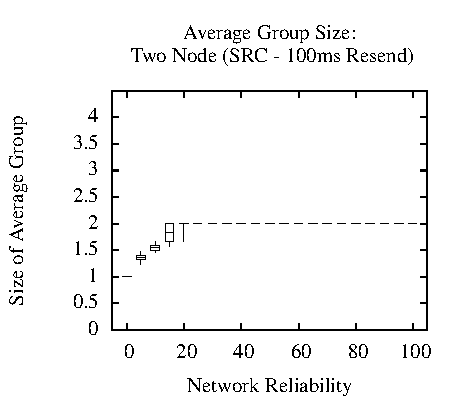
\includegraphics{2NODE-SRC-100-SIZE.pdf}
\caption{Average size of formed groups for two node system with 100ms resend time}
\label{fig:MGS-SRC-2NODE-100}
\end{figure}

\begin{figure}[!h]
\centering
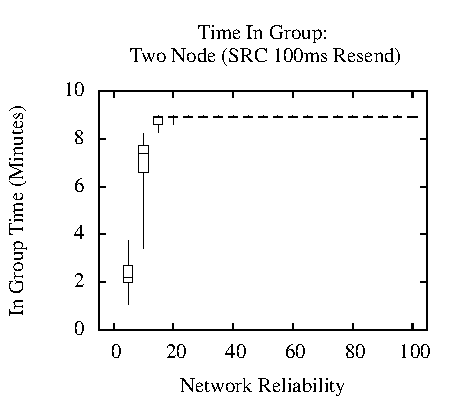
\includegraphics{2NODE-SRC-100-GROUP.pdf}
\caption{Average size of formed groups for two node system with 100ms resend time}
\label{fig:IGT-SRC-2NODE-100}
\end{figure}

The 100ms resend SRC test with two nodes can be considered a sort of a control.
These tests, pictured in Figures \ref{fig:MGS-SRC-2NODE-100} and
\ref{fig:IGT-SRC-2NODE-100}. This test highlights the excellent performance of the
SRC protocol, achieving the maximum in group time of 9 minutes with only 15\%
of datagrams arriving at the receiver. Figure \ref{fig:MGS-SRC-2NODE-100} shows
that when there is no chance of datagrams arriving, the maximum group size is
one since no elections can occur. As the reliability increases, more time is
spent in a group. Since the maximum group size is 2, it is directly related to
the in group time.

\begin{figure}[!h]
\centering
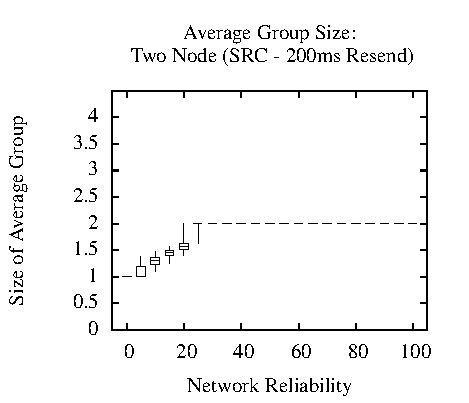
\includegraphics{2NODE-SRC-200-SIZE.pdf}
\caption{Average size of formed groups for two node system with 200ms resend time}
\label{fig:MGS-SRC-2NODE-200}
\end{figure}

\begin{figure}[!h]
\centering
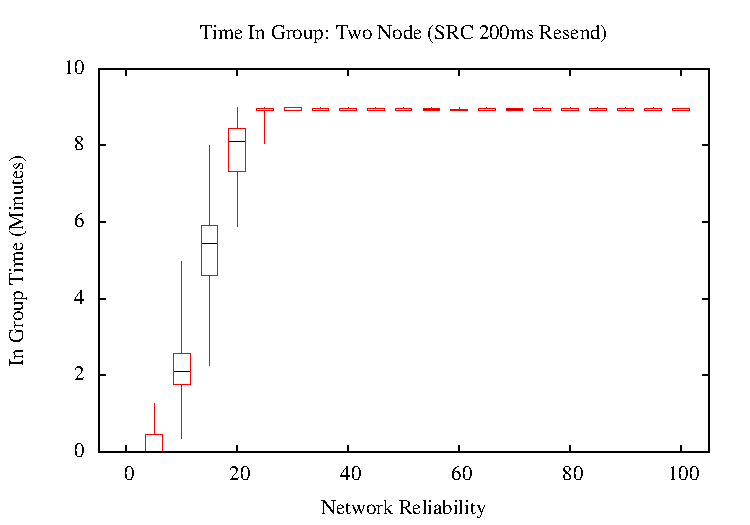
\includegraphics{2NODE-SRC-200-GROUP.pdf}
\caption{Average size of formed groups for two node system with 200ms resend time}
\label{fig:IGT-SRC-2NODE-200}
\end{figure}

Figures \ref{fig:MGS-SRC-2NODE-200} and \ref{fig:IGT-SRC-2NODE-200} demonstrates that as the
rate at which lost datagrams are resent is decreased to resend every 200ms the
time in group falls off. This behavior is expected, since each exchange has a
time limit for each message to arrive and the number of attempts is reduced by
increasing the resend time.

\subsection{Transient Partition Case}

\begin{figure}[!h]
\centering
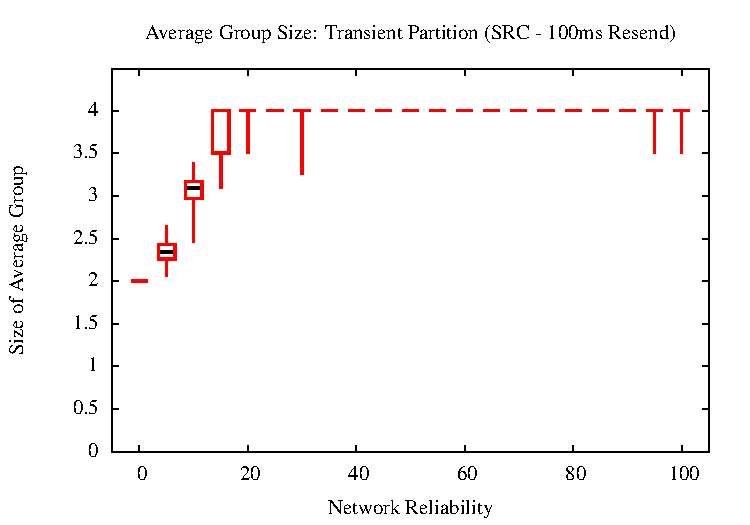
\includegraphics{TRANS-SRC-100-SIZE.pdf}
\caption{Average size of formed groups for the transient partition case with 100ms resend time}
\label{fig:MGS-TRANS-100}
\end{figure}

\begin{figure}[!h]
\centering
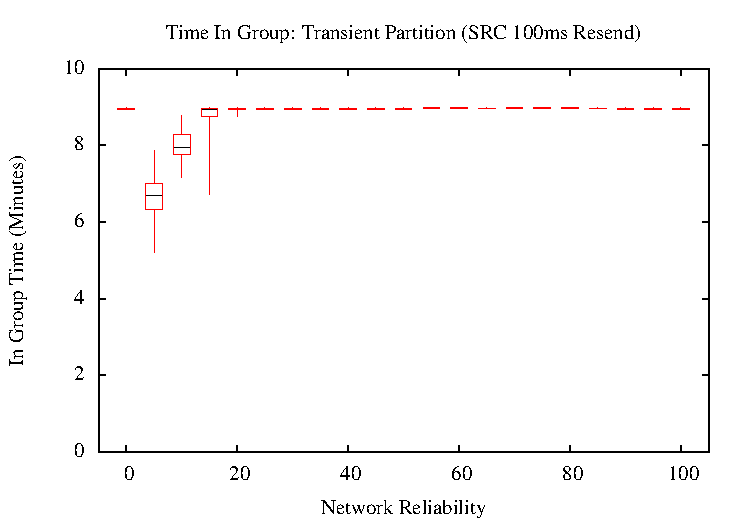
\includegraphics{TRANS-SRC-100-GROUP.pdf}
\caption{Average size of formed groups for the transient partition case with 100ms resend time}
\label{fig:IGT-TRANS-100}
\end{figure}

The transient partition case, shows a simple example where a network partition
separates two groups of DGI. In the simplest case where the opposite side of
the partition is unreachable, nodes will form a group with the other nodes on the
same side of the partition. In our tests, there are two nodes on each side of
the partition. In the experiment, the probability of a datagram crossing the
partition is increased as the experiment continues. The 100ms case is shown in
Figures \ref{fig:MGS-SRC-TRANS-100} and \ref{fig:IGT-SRCTRANS-100}.

While messages cannot cross the partition, the DGIs stay in a group with the
nodes on the same side of the partition leading to an in group time of 9 minutes,
the maximum value. As packets begin to cross the partition (with the reliability
increasing), DGI instances on either side begin to attempt to complete elections
with the nodes on the opposite partition and the time in group begins to fall.
However during this time, the mean group size continues to increase, meaning
while the elections are decreasing the amount of time that the module spends in
state where it can actively do work, it typically does not fall into a state
where it is in a group by itself, which means that most of the lost in group
time comes from elections.

\begin{figure}[!h]
\centering
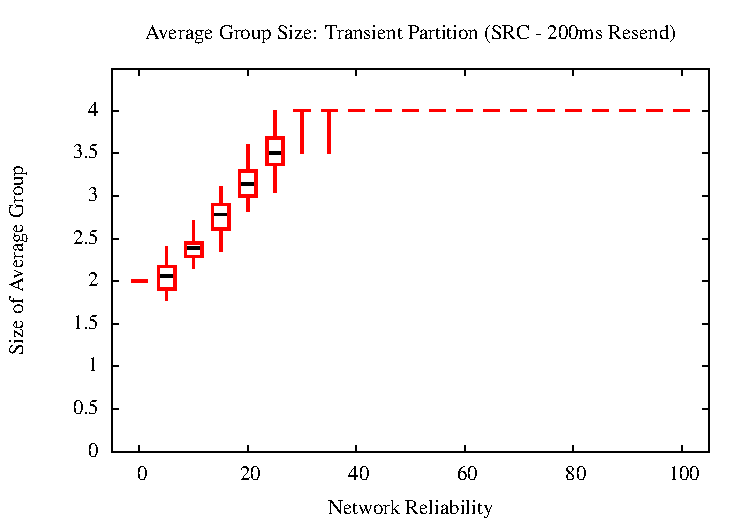
\includegraphics{TRANS-SRC-200-SIZE.pdf}
\caption{Average size of formed groups for the transient partition case with 200ms resend time}
\label{fig:MGS-SRC-TRANS-200}
\end{figure}

\begin{figure}[!h]
\centering
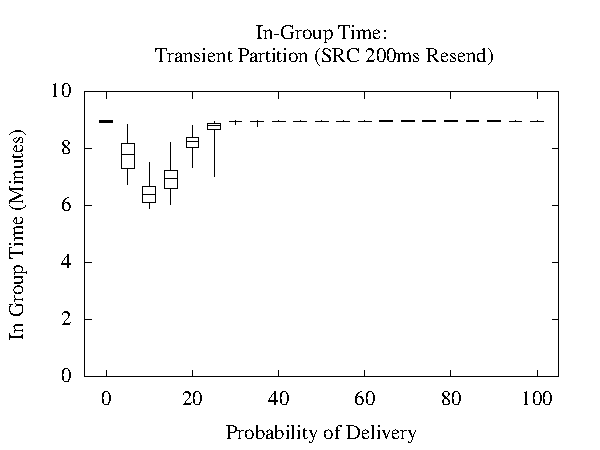
\includegraphics{TRANS-SRC-200-GROUP.pdf}
\caption{Average size of formed groups for the transient partition case with 200ms resend time}
\label{fig:IGT-SRC-TRANS-200}
\end{figure}

The 200ms case, shown in Figures \ref{fig:MGS-SRC-TRANS-200} and \ref{fig:IGT-SRC-TRANS-200} displays similar behavior, with a wider valley due to the
limited number of datagrams. It is also worth noting the that the mean group
size dips below 2 in the figure, possibly because the longer resend times allow
for more race conditions between potential leaders. Discussion of these race
conditions is shown in discussed during the SUC charts since it is more prevalent
in those experiments.

\section{Sequenced Unreliable Connection}

\subsection{Two Node Case}

The SUC protocol's experimental tests show an immediate problem: although there
is a general trend of growth in the amount of time in group and group size
charts, shown in Figures \ref{fig:MGS-SUC-2NODE-100} and \ref{fig:IGT-SUC-2NODE-100}
there is a high degree in variability for any point collected in the experiments.

\begin{figure}[!h]
\centering
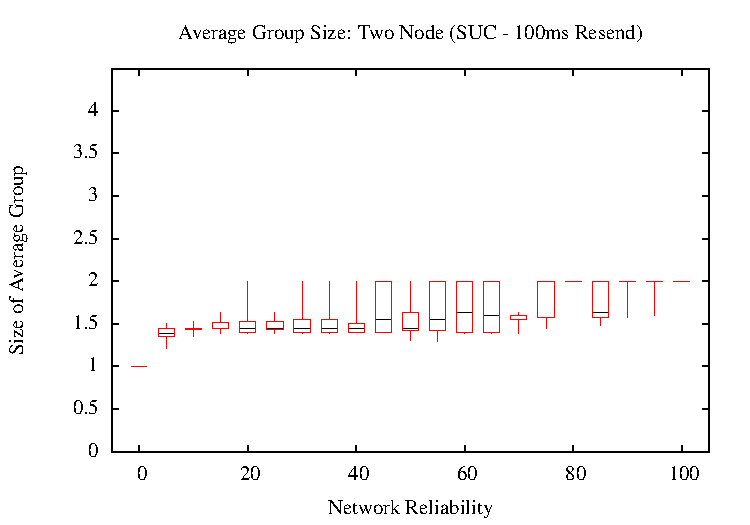
\includegraphics{2NODE-SUC-100-SIZE.pdf}
\caption{Average size of formed groups for two node system with 100ms resend time}
\label{fig:MGS-SUC-2NODE-100}
\end{figure}

\begin{figure}[!h]
\centering
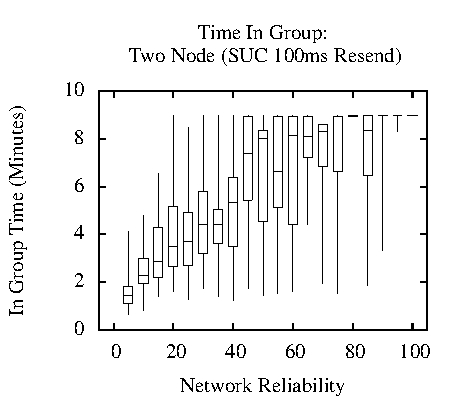
\includegraphics{2NODE-SUC-100-GROUP.pdf}
\caption{Average size of formed groups for two node system with 100ms resend time}
\label{fig:IGT-SUC-2NODE-100}
\end{figure}

In order to identify why these issues occurred, the experimental simulator was
developed. As stated previously, the simulator emulated the packet loss and
behavior of the protocol. The simulator determined the amount of time necessary
to complete and election, and the amount of time that group would last after
being formed. The simulator allowed more trials of each prescribed reliability
and was able to emulate each event at each probability a fixed number of times,
unlike the in the experimental system, where rare events (such as elections
or group failures) were only collected a few times. The collected data was fed
into SharpE.

Using the simulation identified a race condition which is a major factor in the
source of the variability in the collected data. As show in Figure MARK the 
behavior of the algorithm causes the peers to synchronize when there is little
to no latency, as there is in the local area network used to perform the test.
The result is that the coordinators and members attempt to exchange their
keep-alive messages simultaneously. Because the SUC protocol will stop accepting
older sequence numbers when a message is received, race conditions result in
a greater number of lost messages. Since both parties are attempting to
deliver queries and responses, the queries can be destroyed by the responses.
This is a particularly noticeable problem at higher reliability figures. The
probability of a message being lost because a newer message supersedes it
is shown in Figure MARK. (Need to make that one)

The simulator is capable of simulations assume the processes have exact
synchronization, as well has a user defined offset, represented as the number
of ticks for the simulation. A tick of the simulation is the amount of time
that will pass in an experimental run between the time a packet is sent and
the first time that packet is resent (the resend time). In order to accurately
capture the behavoir of a specific experimental run the offset must be estimated
since a changing offset can have a major effect on the characteristics of the
system.

(PROBABLY NEED TO PRODUCE ANOTHER CHART HERE SHOWING HOW OFFSET EFFECTS THE SHAPE OF THE GRAPH).

For the 100ms example, it was estimated that the processes synchronize fairly
closely with each other, and so the simulator was run with a very small offset (approximately 100ms, the smallest the simulator could emulate with one tick)
between the two simulated processes. The result, as compared with the
experimental value is shown in Figure \ref{fig:COMPARE-SUC-2NODE-100}.

\begin{figure}[!h]
\centering
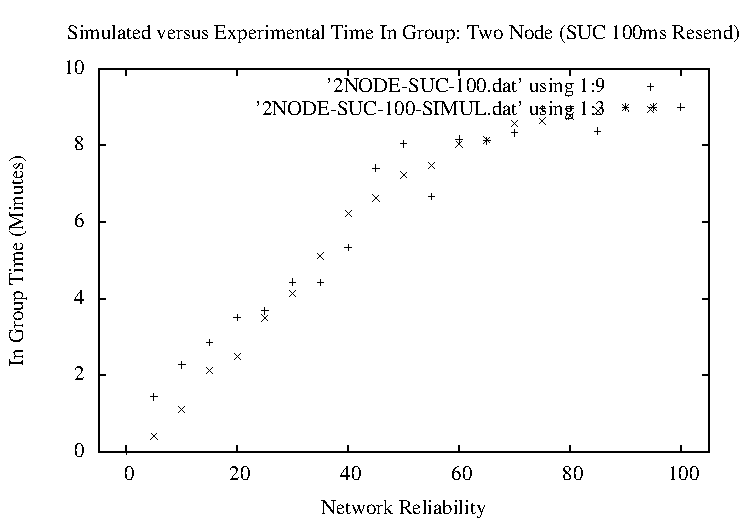
\includegraphics{2NODE-SUC-100-COMPARE.pdf}
\caption{Comparison of in group time as collected from the experimental platform and the simulator (1 tick offset between processes).}
\label{fig:COMPARE-SUC-2NODE-100}
\end{figure}

From figures \ref{fig:COMPARE-SUC-2NODE-100} and MARK one can conclude that for the SUC protocol the 
race condition between processes is a major factor in the amount of time processes
can spend in groups. While it is obvious that competition for access to the channel
is a detriment to the system, the replication of this competition in software is
also a major factor in the stability of groups formed. Furthermore, based on the 
real-time design of the DGI, synchronization is a major concern because the real-time
execution is designed to cause the processes to synchronize as closely as possible.

\begin{figure}[!h]
\centering
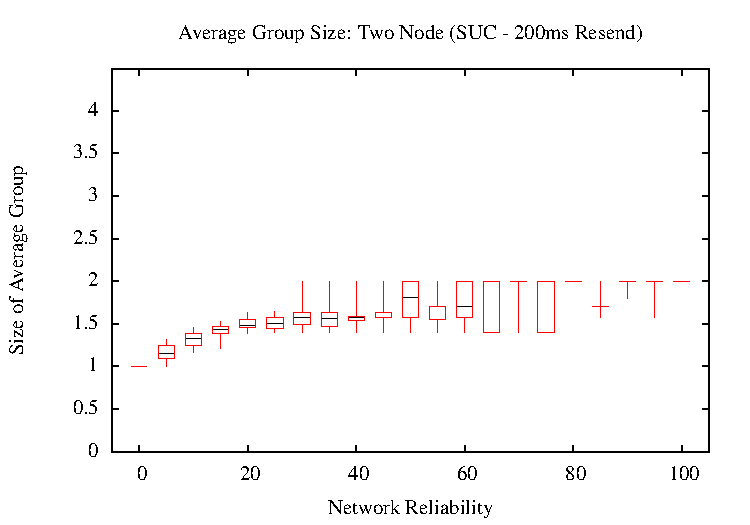
\includegraphics{2NODE-SUC-200-SIZE.pdf}
\caption{Average size of formed groups for two node system with 200ms resend time}
\label{fig:MGS-SUC-2NODE-200}
\end{figure}

\begin{figure}[!h]
\centering
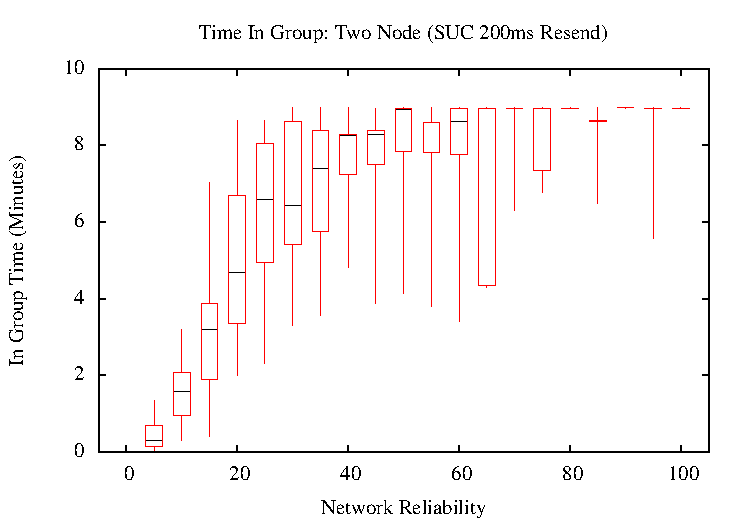
\includegraphics{2NODE-SUC-200-GROUP.pdf}
\caption{Average size of formed groups for two node system with 200ms resend time}
\label{fig:IGT-SUC-2NODE-200}
\end{figure}

\begin{figure}[!h]
\centering
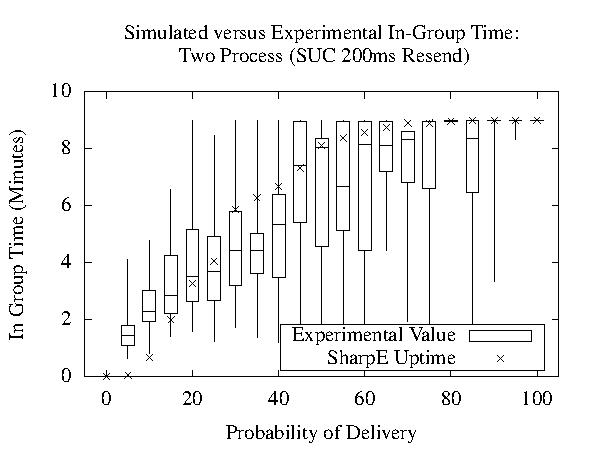
\includegraphics{2NODE-SUC-200-COMPARE.pdf}
\caption{Comparison of in group time as collected from the experimental platform and the simulator (2 tick offset between processes).}
\label{fig:COMPARE-SUC-2NODE-200}
\end{figure}


In the 200ms resend case, show in Figures \ref{fig:MGS-SUC-2NODE-200} and \ref{fig:IGT-SUC-2NODE-200}, we can observe a more consistent and
growth rate in the in group time as a the reliability increases. In fact, averaging
across all the collected data points from the experiment, the average in group time
is higher for the 200ms case than it is for the 100ms case ( 6.86 vs 6.09 ). Once
again, race conditions are the culprit: the collected data when fit to a run of the
simulation corresponds to a greater offset in the simulator: approximately 400ms (2 ticks at 200ms),
which is two ticks of the stimulation. The comparison between the experimental and
simulator values is shown in Figure \ref{fig:COMPARE-SUC-2NODE-200}.

